\chapter{Neural Posterior Unfolding}
\label{chap:npu}
\section{Motivation for improved binned unfolding}
    A binned unfolding method is one in which both the particle--level and detector--level distributions are discretised into histograms, transforming the continuous convolution of \cref{eq:forward-folding} into the matrix equation \cref{eq:forward-binned}.

\subsection{Degeneracy and Null Spaces in Unfolding}
    One of the fundamental challenges in unfolding collider data comes from degeneracies in the response matrix.
    %
    Consider a case where two particle level bins $\alpha$ and $\beta$ are indistinguishable at the detector level.
    %
    This statement can be formalised as, there exists a detector level bin $\kappa$ such that for all detector level bins $\iota$:
    \begin{equation}
        R_{\iota\alpha} = R_{\iota\beta} = \delta_{\iota\kappa}
    \end{equation}
    where $\delta$ is the Kronecker delta.
    %
    In such scenarios, traditional methods like Iterative Bayesian Unfolding (IBU) produce catastrophically poor results, because the unfolded result becomes entirely dependent on the simulation, and learns no information from the data.
    %
    The update rule for IBU takes the form
    \begin{equation}
        \forall n \in \mathbb{N}
        \qquad
        \nu_{\alpha}^{(n)} = \left(\frac{\nu_\alpha^{(0)}}{\nu_\alpha^{(0)} + \nu_{\beta}^{(0)}}\right) \cdot \mu_\kappa
        \qquad
        \nu_{\beta}^{(n)} = \left(\frac{\nu_\beta^{(0)}}{\nu_\alpha^{(0)} + \nu_{\beta}^{(0)}}\right) \cdot \mu_\kappa\,.
    \end{equation}

    This means the relative contributions of bins $\alpha$ and $\beta$ to the unfolded result are entirely determined by the MC, regardless of the observed data.
    %
    Even worse, IBU (with, e.g., bootstraps) will report zero uncertainty on the ratio \(\nicefrac{\nu_\alpha}{\nu_\alpha+\nu_\beta}\) when in reality this ratio should have maximal uncertainty since the detector cannot distinguish between these contributions.
\subsection{Regularization Limitations}
    To address the ill-posedness detailed in Sec.~\ref{sec:ill-posed}, traditional methods employ various forms of regularisation, examples of which are provided in Sec.~\ref{sec:binned-methods}.
    %
    However, all these approaches require a careful balance between fidelity to the data and conformity to the regularisation constraints.
    %
    These methods typically do not provide a natural framework for propagating uncertainties and can significantly underestimate the true uncertainty in degenerate regions.
    %
    These limitations motivate the development of new unfolding methods that can
    \begin{enumerate}
        \item Naturally handle degeneracies and null spaces in the response matrix,
        \item Provide proper uncertainty quantification, especially in poorly constrained regions,
        \item Reduce dependence on arbitrary regularization parameters, and
        \item Offer computational efficiency for large-scale problems.
    \end{enumerate}
    \emph{Neural Posterior Unfolding}~\cite{acosta2024npu} addresses these challenges head on, by leveraging normalising flows for neural posterior estimation~\cite{Papamakarios2016FastEstimation}.
    %
    Unlike traditional methods that provide point estimates, NPU yields a full posterior distribution over the unfolded parameters, naturally capturing uncertainties in poorly constrained regions. 
    %
    Additionally, the regularisation in NPU emerges implicitly from the neural network architecture and training protocol, reducing the need for manual tuning of regularization parameters.

    In the following sections, we introduce normalising flows and neural posterior estimation as the foundation for the NPU method, demonstrating how these modern machine learning techniques address the fundamental challenges of binned unfolding.
\section{Normalising flows for inverse problems.}
\subsection{A Bayesian perspective on inverse problems.}
    The unfolding problem can be naturally framed in Bayesian terms.
    %
    Given detector level measurements \(x\), we aim to reconstruct the posterior distribution over particle level quantities \(z\),
    \[
        \label{eq:bayes-theorem}
        p(z\,|\,x) = \frac{p(x\,|\,z)\,p(z)}{p(x)}
    \]
    Where $p(x\,|\,z)$ is the detector response, \(r(x\,|\,z)\), $p(z)$ is the prior for particle level quantities, and $p(x)$ is the evidence.
    %
    Traditional methods typically focus on finding a point estimate that maximises this posterior, but a full Bayesian treatment would characterize the entire posterior distribution to properly account for uncertainties and degeneracies.

    Normalising flows offer several key advantages for modelling the posterior distribution in inverse problems.
    \begin{itemize}
        \item \textbf{Complex distribution modelling:} Unlike standard parametric approaches, normalising flows can represent multimodal, asymmetric posteriors that often arise in inverse problems with degeneracies where multiple particle level configurations can lead to similar detector level observations.
        \item \textbf{Amortised inference}: Once trained, normalising flows enable rapid posterior sampling without requiring new optimization runs for each new observation.
            This is particularly valuable when processing large datasets or when rerunning statistical analyses with different systematic variations.
        \item \textbf{End to end differentiability}: The entire posterior estimation process can be optimized end to end, enabling gradient based learning approaches that are more efficient than traditional MCMC methods for high dimensional unfolding.
        \item \textbf{Implicit regularization}: Neural network architectures naturally introduce an inductive bias that serves as implicit regularisation, potentially reducing overfitting to statistical fluctuations compared to direct matrix inversion approaches without requiring explicit regularisation parameters.
    \end{itemize}
\subsection{Conditional normalising flows for inverse problems.}
    In the context of unfolding, we're particularly interested in modelling the conditional distribution $p(z\,|\,x)$, the particle--level distribution given detector--level observations.
    %
    Conditional normalising flows, described in \cref{subpar:conditional-nfs} an architecture almost perfectly designed for this task.
    %
    A flow \(f_\theta\) with learnable parameters \(\theta\) can be trained to model the particle level distribution \(z\),
    \[
        z = f_\theta(u\,|\,y),
    \]
    where $u$ is drawn from a simple base distribution\footnote{typically a standard normal}, and $x$ is the conditioning variable, detector level data.
    %
    This conditional structure allows the flow to learn the posterior distribution specifically tailored to each detector level observation, capturing the uncertainty and potential multimodality of the solution even in regions where the detector response is non injective.

    While Markov Chain Monte Carlo (MCMC) methods have traditionally been used for Bayesian inference in inverse problems~\cite{Kaipio2005StatisticalProblems, Segura2024APhysics, Dashti2017TheProblems, 2005InverseMeasurements, 2005StatisticalTheory}\footnote{As they are in Fully Bayesian Unfolding~\cite{choudalakis_fully_2012}}, normalising flows have some unique properties that make them especially well suited to this task.
    \begin{enumerate}
        \item  No burn in period is required once the flow is trained,
        \item Samples are generated independently rather than in a correlated chain,
        \item The computational cost of generating samples does not increase with the dimensionality of the parameter space, and perhaps most importantly,
        \item Due to the fully differentiable structure of the network, training can leverage GPU acceleration and parallelisation.
    \end{enumerate}
    
    These advantages make normalising flows particularly attractive for inverse problems where MCMC methods may face mixing and convergence challenges or become computationally prohibitive to use.
\section{The Neural Posterior Unfolding Algorithm}
    Neural Posterior Unfolding (NPU) is a novel approach to unfolding that combines the rigour of Bayesian statistics with the flexibility and computational efficiency of modern machine learning.
    %
    Rather than focusing solely on point estimates, NPU aims to characterise the full posterior distribution over particle level observables, providing comprehensive uncertainty quantification while addressing the key limitations of traditional unfolding methods.
\subsection{Statistical foundation}
    At its core, NPU leverages normalising flows for neural posterior estimation in the context of binned unfolding.
    %
    The fundamental insight is to directly estimate the conditional posterior distribution \(p(z\,| \,x)\) through \(P(\vb*\nu\,|\, \vb*\mu)\) the probability that the true particle level histogram counts are $\vb*\nu$ given the measured detector level histogram counts are $\vb*\mu$.

    The relevant statistical quantities are
        \begin{itemize}
        \item A detector level histogram $\vb*\mu = \{\mu_j\}_{j=1}^{N_D}$, where $\mu_j$ is the number of events in detector level bin $j$
        \item A particle level histogram $\vb*\nu = \{\nu_i\}_{i=1}^{N_T}$, where $\nu_i$ is the number of events in particle level bin $i$
        \item A response matrix $\mathbf{R}$ with elements $R_{ji} = P(\mu_j|\nu_i)$, the probability of an event in particle level bin $i$ being measured in detector level bin $j$
    \end{itemize}
    The forward model relating these quantities is given by \cref{eq:forward-binned}.
    %
    In this framework the posterior distribution of \cref{eq:bayes-theorem} is approximated by
    \[
        P(\vb*\nu\,|\,\vb*\mu) = \frac{P(\vb*\mu\,|\,\vb*\nu)\,P(\vb*\nu)}{p(\vb*\mu)}
    \]
    where $P(\vb*\mu\,|\,\vb*\nu)$ is the likelihood, $p(\vb*\nu)$ is the prior, and $p(\vb*\mu)$ is the evidence.
    %
    For Poisson distributed measurements, the likelihood takes the form
    \[
        P(\mu|\nu) = \prod_{j=1}^{N_D} \frac{(\sum_i R_{ji}\nu_i)^{\mu_j} e^{-\sum_i R_{ji}\nu_i}}{\mu_j!}
    \]
    
    NPU is conceptually similar to Fully Bayesian Unfolding (FBU), but replaces the traditional Markov Chain Monte Carlo (MCMC) sampling with normalising flows for neural posterior estimation, providing computational advantages and increased flexibility while maintaining the same full Bayesian treatment of the problem~\cite{Rezende2015VariationalFlows}.
\subsection{Machine Learning Architecture}
    NPU builds upon the neural posterior estimation framework, which uses conditional normalising flows to directly model the posterior distribution.
    %
    The NPE framework comprises the base distribution, a simple distribution $p_u(u)$ that is easy to sample from,
    %
    an invertible transformation, a learnable, invertible function $f_\theta(u|\vb*\mu)$ that transforms samples from the base distribution into samples from the approximate posterior, conditioned on the measured data $\vb*\mu$, and
    %
    a density transformation, encoding the the change of variables formula,
    \[
        P_\theta(\vb*\nu\,|\,\vb*\mu) = P_u(f_\theta^{-1}(\vb*\nu\,|\,\vb*\mu)) \left|\det\qty{ \grad_{\vb*\nu}f_\theta^{-1}(\vb*\nu\,|\,\vb*\mu)}\right|
    \]
    The neural network parameters $\theta$ are optimized to maximize the likelihood of the true posterior, using pairs of simulated $(\nu_i, \mu_j)$ examples.
    %
    The training objective is to minimize the loss function
    \[
        \label{eq:nf-nll}
        \mathcal{L}(\theta) = -\mathbb{E}_{(\vb*\mu,\vb*\nu) \sim P_{\text{sim}}(\vb*\nu, \vb*\mu)} \big[ \log P (\vb*\nu\,|\,\vb*\mu)\big]
    \]
    This approach allows the model to learn complex posterior distributions, including multimodal and highly correlated structures that often arise in unfolding problems~\cite{Papamakarios2016FastEstimation}.

    In practical implementations, uses a normalizing flow based on the MADE (Masked Autoencoder for Distribution Estimation) architecture~\cite{papamakarios_masked_2018}.
    %
    The network is made up of an invertible transformation network with three fully connected layers, each containing \(50-100\) nodes with Swish activation functions~\cite{Ramachandran2017SearchingFunctions}.
    %
    Conditional inputs incorporated through an auxiliary fully connected layer.
    %
    The network is then trained for \(1000-1500\) epochs using the \textsc{Adam} optimiser with a learning rate of \(\num{d-4}\) and a batch size of \(\num{d4}\).
    %
    The loss function is the negative log likelihood described above in \cref{eq:nf-nll}.
    
    This architecture provides sufficient flexibility to model complex posterior distributions while remaining computationally tractable~\cite{Rezende2015VariationalFlows, Kobyzev2019NormalizingMethods}.
    %
    After training the normalising flow, the unfolded response is obtained through a Maximum Likelihood Estimation (MLE) step, where the negative log likelihood of the observed data conditioned on the learned model is minimised.
    %
    This optimisation process also uses the same \textsc{Adam} optimiser.
\subsection{Addressing degeneracy with NPU.}
    A major advantage of NPU over traditional unfolding methods is its ability to naturally handle degeneracies in the response matrix.
    %
    Consider the two bin degenerate example presented earlier, where two particle level bins $\alpha$ and $\beta$ are indistinguishable at the detector level.
    %
    In traditional methods like IBU, the unfolded result becomes entirely dependent on the prior and incorrectly report zero uncertainty on the ratio \(\nicefrac{\nu_\alpha}{\nu_\alpha+\nu_\beta}.\)

    In contrast, NPU naturally returns a broad posterior distribution that properly reflects the uncertainty.
    %
    This is demonstrated in~\cite{acosta2024npu} with a two bin example where the response becomes increasingly degenerate, with correlation coefficient \(\rho\to 1\).
    %
    As the detector loses its ability to differentiate between truth bins, NPU produces credible intervals that encompass all values consistent with the total counts, appropriately reflecting the inherent uncertainty.
    %
    Simultaneously, while allowing for uncertainty in degenerate directions, NPU maintains constraints in well determined directions, such as the total sum $\nu_\alpha + \nu_\beta$.
    %
    This behaviour emerges naturally from the Bayesian formulation, without requiring explicit identification of the degenerate subspaces.
    %
    By modelling the full posterior, NPU provides a principled way to represent uncertainty in precisely those directions where the data provides little or no constraint.

\subsection{Implicit regularisation in NPU.}
    A significant advantage of NPU is its implicit regularisation, which arises naturally from the neural network architecture and training procedure rather than requiring explicit regularisation terms or early stopping rules.
    %
    Several mechanisms contribute to this implicit regularization.
    \begin{itemize}
        \item \textbf{Network capacity}: The finite capacity of the neural network limits the complexity of the posterior approximation, preventing overfitting to statistical noise in a manner similar to how traditional regularisation constrains solution complexity.
        \item \textbf{Smooth transformations}: Normalising flows use smooth transformation functions, which naturally bias the solution toward smooth posterior distributions rather than ones with sharp, unphysical features.
        \item \textbf{Amortized inference}: By learning a conditional distribution that applies across many possible measurements, NPU averages over many training examples, reducing sensitivity to outliers or statistical fluctuations in any single measurement.
        \item \textbf{Architectural inductive bias}: The specific architecture of the normalising flow introduces an inductive bias.
        %
        For instance, MADE architectures model dependencies between variables in a structured way that can align with physical correlations between bins.
        \item \textbf{Optimisation dynamics}: The stochastic gradient descent training process itself provides regularisation through early stopping based on validation performance, preventing overfitting to the training data.
    \end{itemize}
    This implicit regularisation offers some advantages over the explicit regularisation used in traditional methods.
    %
    It adapts automatically to the complexity of the problem rather than requiring manual tuning of regularization parameters,
    %
    it can handle different degrees of regularisation for different regions of the solution space, providing stronger regularisation where constraints are weak and less regularisation where data provides strong constraints, and
    it emerges from general principles rather than specific assumptions about the solution\footnote{such as smoothness or proximity to a prior}, potentially leading to less biased results.
    %
    The effectiveness of this implicit regularisation can be observed empirically in cases where NPU produces unfolded distributions with excellent agreement with the truth, despite the ill--posed nature of the problem.

    The next section will demonstrate the application of NPU to concrete examples, including both controlled Gaussian distributions and realistic jet substructure measurements, to illustrate its performance in practice.
\section{Numerical results.}
    This section presents comprehensive empirical validation of Neural Posterior Unfolding (NPU) through a series of increasingly complex examples.
    %
    Let us first consider a simple two--bin degenerate case to illustrate NPU's advantages in handling unconstrained regions of phase space, then move to a Gaussian example to systematically assess statistical performance, and finally study the method's efficacy on realistic jet substructure simulation from the LHC.
    \subsection{2 bin degenerate response example.}
        Our first example illustrates NPU's behaviour by honing in degenerate scenarios where traditional methods struggle.
        %
        We construct a two--bin setup where $t, m \in \mathbb{R}^2$ with a response matrix $\mathbf{R} \in \mathbb{R}^{2 \times 2}$.
        %
        We fix the truth values at $\nu_0 = \nu_1 = 5 \times 10^4$ and parametrise the response matrix using a correlation coefficient $\rho$ and diagonal elements $\sigma_0 = \sigma_1 \equiv \sigma = 0.8$.

When $\rho = 0$, the response matrix is well conditioned with a nearly diagonal structure, meaning each detector bin primarily receives contributions from a single truth bin.
%
In this scenario, both IBU, with uncertainty quantification via bootstrapping, and NPU yield unfolded distributions that align well with the truth, producing statistically consistent confidence regions.
%
These results are demonstrated in \cref{fig:2bin:a}, where both methods successfully recover the true distribution within their respective uncertainty bands.

However, when the response matrix becomes degenerate, i.e., $R_{i\alpha} = R_{i\beta}$, the detector loses its ability to differentiate between the two truth bins.
%
This degeneracy means that multiple truth configurations can produce identical detector level observations, making the unfolding problem underconstrained.
%
Under these conditions, IBU struggles with the ill-posed nature of the problem.
%
It provides only a point estimate based entirely on the prior distribution, while incorrectly estimating zero uncertainty for the ratio $\nicefrac{\nu_\alpha}{\nu_\alpha+\nu_\alpha}$.
%
This failure to capture the true uncertainty is a inescapable limitation of IBU when dealing with degenerate responses.
%
In stark contrast, NPU handles this degeneracy gracefully by returning a full posterior distribution with credible intervals that appropriately span all values consistent with the observed total counts.
%
This behaviour accurately reflects the inherent uncertainty and ambiguity of the degenerate unfolding problem, as demonstrated in \cref{fig:2bin:b}.
%
The NPU approach thus provides a more honest and statistically sound treatment of cases where the data cannot uniquely determine the truth distribution.

\begin{figure}
    \centering
    \subfloat[2 bin example with non degenerate response]{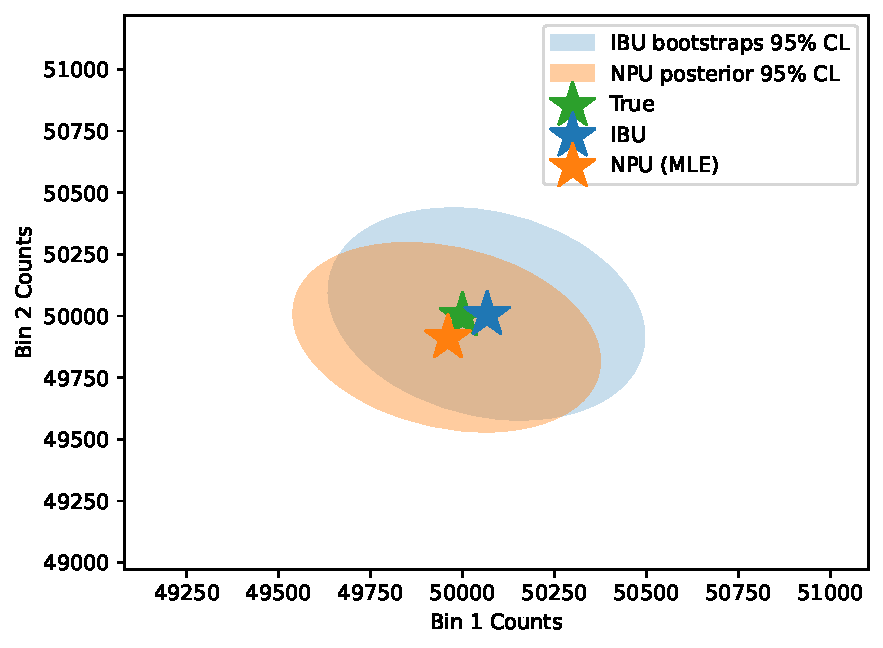
\includegraphics[width=0.485\textwidth]{figures/chapter-04/2bin_95CL.pdf}\label{fig:2bin:a}}
    \subfloat[2 bin example with degenerate response]{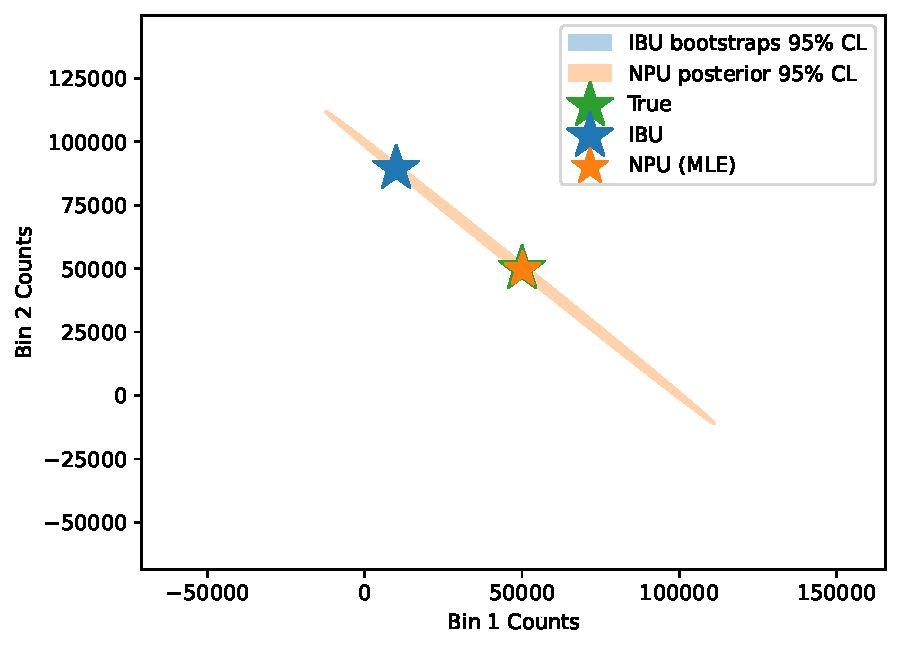
\includegraphics[width=0.49\textwidth]{figures/chapter-04/2bin_degenerateResp.pdf}\label{fig:2bin:b}}
    \caption[2 bin example]{Comparison between NPU and IBU using a two bin example.
    %
    The MLE estimate of NPU is shown with an orange star, the IBU prediction with a blue star, and the true value with a green star.
    %
    The orange and blue shaded regions represent the 95\% credible intervals of NPU and IBU, respectively.
    %
    \textbf{(a)} Non degenerate, nearly diagonal response matrix $(\rho = 0)$: 
    Both IBU and NPU yield unfolded distributions that agree well with the truth.
    %
    \textbf{(b)} Degenerate response $(R_{i\alpha} = R_{i\beta})$: 
    IBU relies solely on the prior, while NPU produces a full posterior with credible intervals that properly account for uncertainty in unconstrained regions.
    The NPU maximum likelihood estimate closely aligns with the true distribution, and the NPU posterior is compatible with the statistical uncertainty evaluated by IBU using bootstraps.\protect{\footnotemark}
    }
    \label{fig:2bin}
\end{figure}
\footnotetext{Figure created by Jingjing Pan.}

        This example highlights a fundamental advantage of NPU and other Bayesian methods;
        %
        they naturally capture uncertainty in unconstrained regions of phase space, while traditional methods like IBU can dramatically underestimate uncertainties when degeneracies are present.
\subsection{Gaussian example.}
    The second test employs a Gaussian distribution with known truth, allowing one to systematically evaluate NPU's performance with varying levels of detector smearing. 
    \subsubsection{Experimental setup}
Generate two from identical one dimensional Gaussian distributions with mean $\mu = 0$ and standard deviation $\sigma = 1$,
a generation dataset ({Gen.}) with $\num{d6}$ events for training, and a truth dataset ({Truth}) with $\num{d5}$ events for validation.

To simulate detector effects, apply Gaussian smearing with parameter $\epsilon = 0.5$ to both particle level datasets.
%
This produces corresponding detector level distributions, {Sim.}, from Gen., and {Data}, from Truth), both with the same mean but with increased width $\sigma_\text{detector} = \sqrt{1^2 + 0.5^2} \approx 1.12$.
%
The response matrix $\mathbf{R}$ is estimated from (Gen., Sim.) pairs.
%
This response matrix is then used to unfold the observed Data, with results compared against the known Truth.
%
The experimental setup and resulting response matrix are shown in \cref{fig:gaus_init}.
\begin{figure}
    \centering
    \subfloat[Experimental setup]{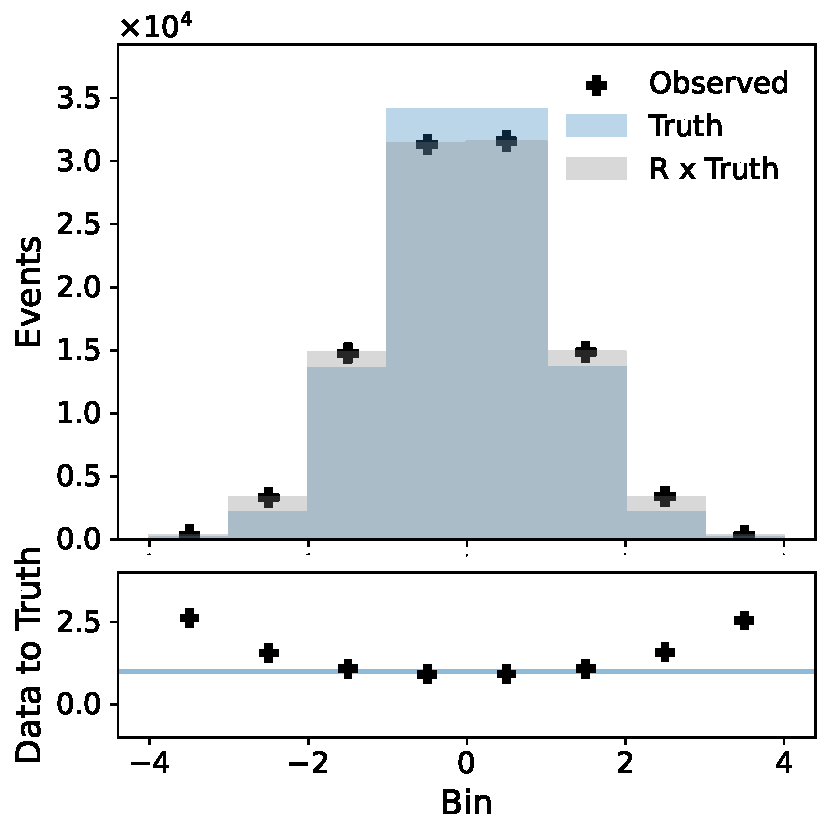
\includegraphics[width=0.45\textwidth]{figures/chapter-04/gaus_init.pdf}\label{fig:gaus_init:a}} 
    \subfloat[Response matrix]{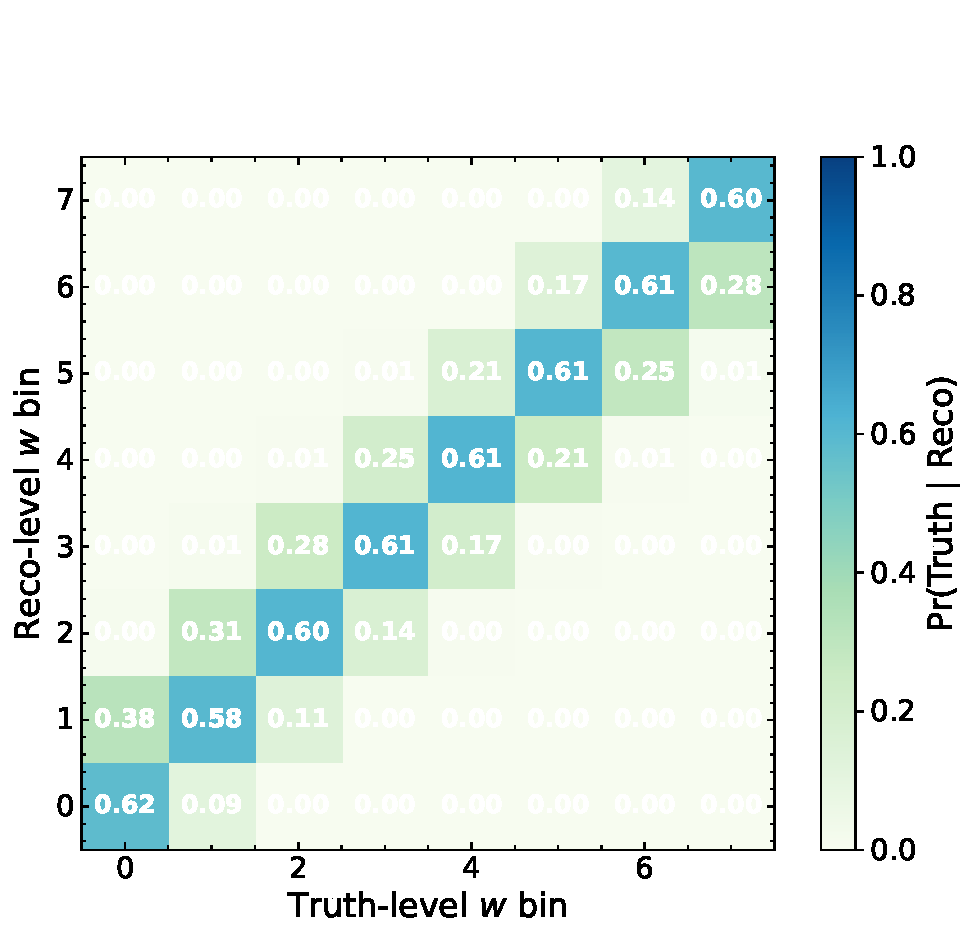
\includegraphics[width=0.535\textwidth]{figures/chapter-04/gaus_resp.pdf}\label{fig:gaus_init:b}} \\
    \caption[Gaussian example setup]{Gaussian unfolding example setup. 
    \textbf{(a)} The experimental design: Truth (blue) represents the target particle-level Gaussian distribution to be recovered, while Data (black crosses) shows the corresponding detector-level observations after Gaussian smearing. 
    %
    The goal of unfolding is to recover the Truth distribution from the observed Data.
    \textbf{(b)} The response matrix $\mathbf{R}$ constructed from Gen./Sim. pairs, which encodes the detector smearing transformation and serves as an input for the unfolding algorithms.
    %
    The matrix shows how probability mass spreads from each particle level bin (horizontal axis) to detector level bins (vertical axis).\footnotemark
    }
    \label{fig:gaus_init}
\end{figure}
\footnotetext{Figure created by Jingjing Pan.}
\subsubsection{Results and comparison}
    The unfolded distributions from NPU (Maximum Likelihood Estimate), IBU, and FBU all accurately recover the truth distribution, as shown in \cref{fig:gaus:a}.
    %
    Beyond point estimates, NPU provides a complete characterization of the uncertainty through its full posterior distribution, including bin-to-bin correlations visible in the corner plot in \cref{fig:gaus:b}.
    %
    This corner plot reveals the pairwise relationships between bins and demonstrates strong agreement between the posterior distributions from NPU and FBU, with both methods properly encompassing the true distribution.
\begin{figure}
\centering
\subfloat[Unfolded distributions]{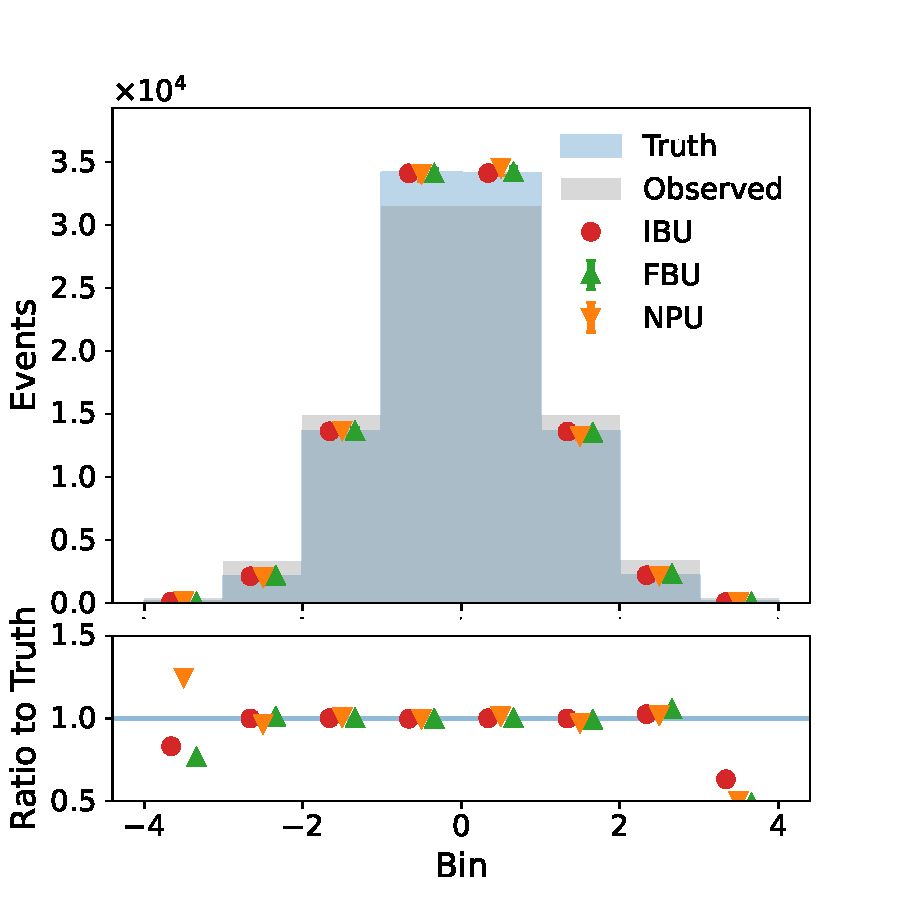
\includegraphics[width=0.48\textwidth]{figures/chapter-04/npu_gaussian_smearing_0.5.pdf}\label{fig:gaus:a}} 
\subfloat[Posterior correlations]{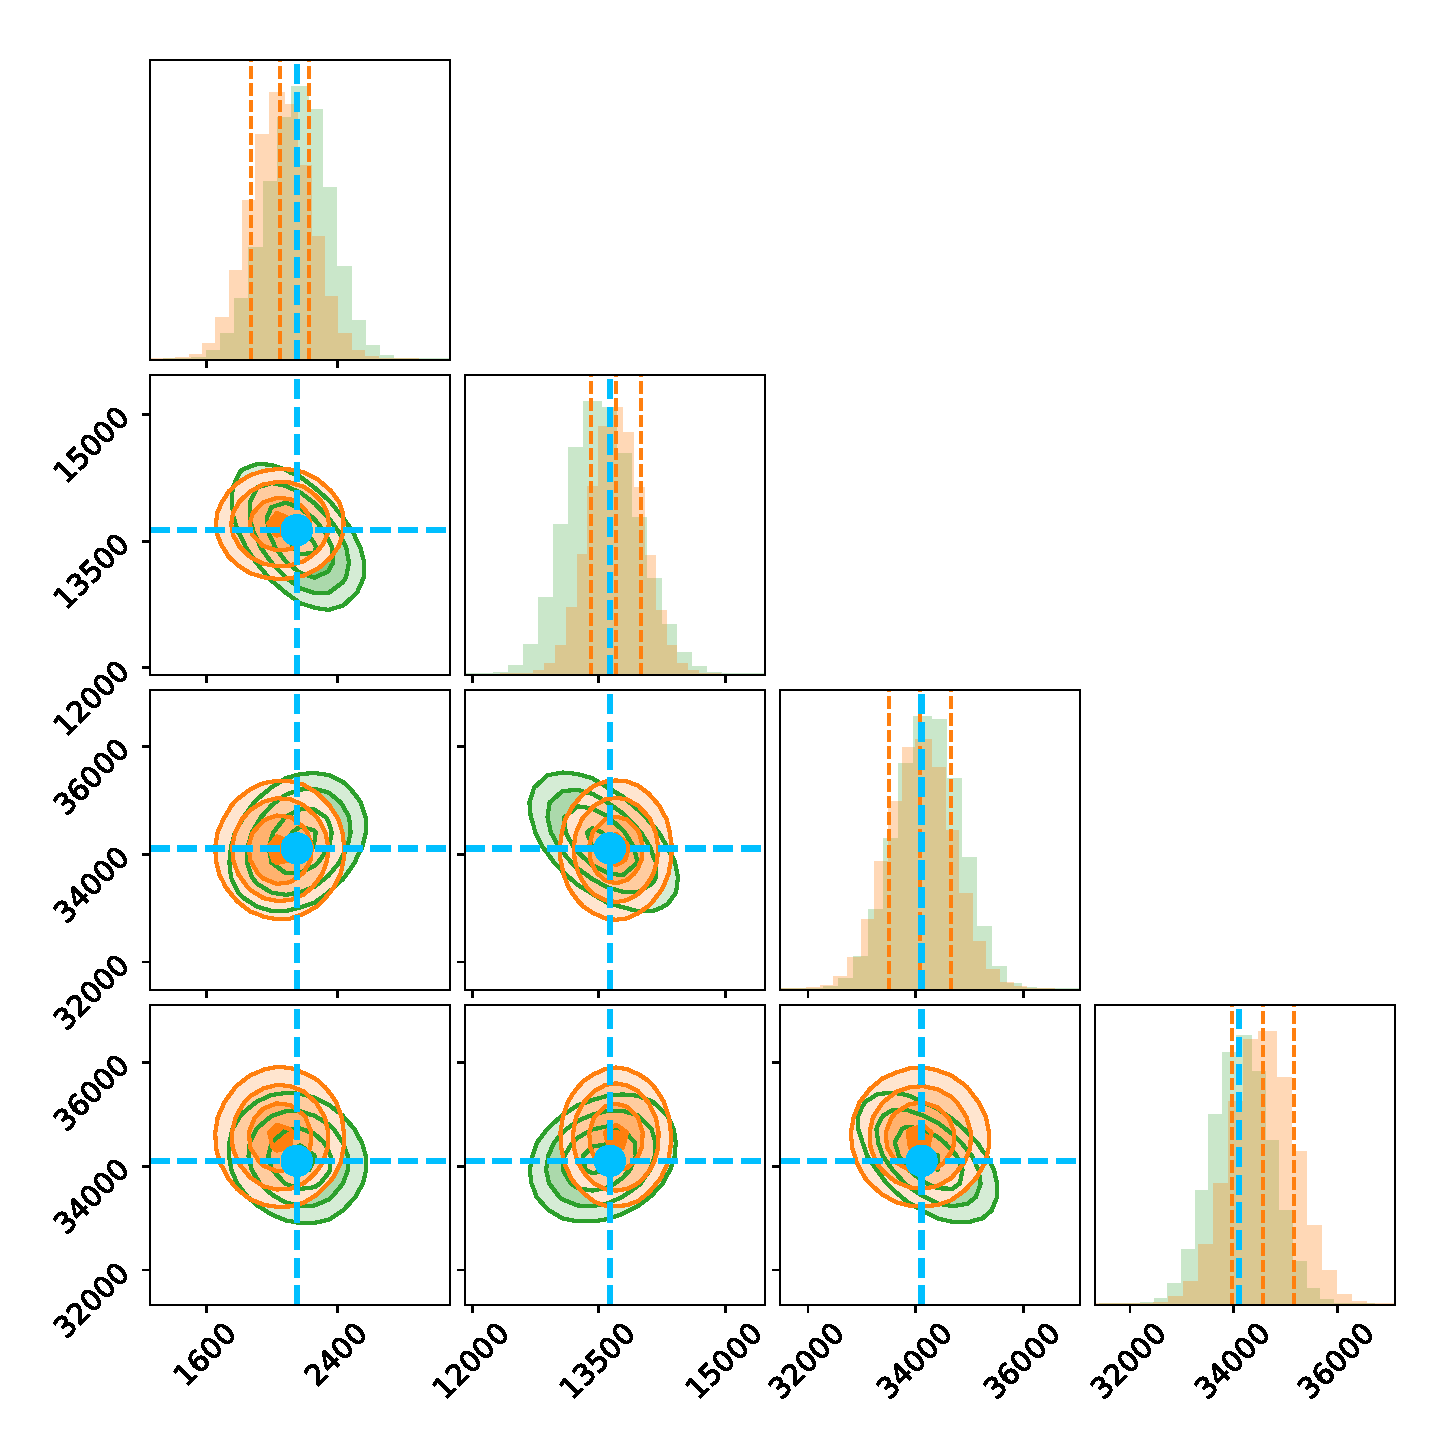
\includegraphics[width=0.48\textwidth]{figures/chapter-04/gaus_corner.pdf}\label{fig:gaus:b}} \\
\caption[Gaussian unfolding results and posterior analysis]{Gaussian unfolding results comparison.
\textbf{(a)} Unfolded distributions: NPU MLE (orange down triangles), IBU (red circles), and FBU (green up triangles) compared with truth (blue shaded region).
%
All methods successfully recover the true distribution.
%
\textbf{(b)} Corner plot showing pairwise posterior correlations between the four central bins from NPU (orange contours) and FBU (green contours, averaged over MCMC samples), with truth values marked in blue. 
Both methods show consistent posterior distributions that properly encompass the true values.
%
The green for FBU is averaged over many draws.\footnotemark
}
\label{fig:gaus}
\end{figure}
\footnotetext{Figure created by Jingjing Pan.}

    To rigorously assess the statistical calibration of NPU, evaluate pull distributions across 100 pseudo experiments.
    %
    For each bin $i$ in pseudo experiment $j$, compute the standardised residual:
    \[
        \text{Pull}_{ij} = \frac{\mu^{\text{method}}_{ij} - \nu_i}{\sigma^{\text{method}}_{ij}}
    \]
    where $\mu^{\text{method}}_{ij}$ and $\sigma^{\text{method}}_{ij}$ are the posterior mean and standard deviation for that bin, and $\nu_i$ is the true value.
    
    Recall from \cref{subsubsec:pull-distributions} that for properly calibrated uncertainty estimates, these pulls should follow a standard normal distribution with zero mean and unit variance.
    %
    As demonstrated in \cref{fig:pulls:a}, the pull distributions for both NPU and FBU with moderate smearing ($\epsilon = 0.5$) are indeed well centred at zero with unit width, confirming proper statistical calibration.
    %
    One can further tested the robustness of this calibration by varying the smearing parameter across $\epsilon \in [0.3, 0.6]$, finding that both methods maintain proper coverage throughout this range.
    %
    \cref{fig:pulls:b} 
\begin{table}
\centering
\caption[Computational cost comparison between FBU and NPU]{Computational cost comparison between FBU and NPU for repeated unfolding tasks. NPU's amortised inference approach provides significant speed-up despite the initial training overhead.}
\vspace{3mm}
\label{tab:timing}
\begin{tabular}{|l|c|c|c|}
\hline
\textbf{Method} & \textbf{Setup cost} & \textbf{Per run} & \textbf{Total (100 runs)} \\
\hline
FBU (10k MCMC draws) & -- & 40 sec & $\sim$67 min \\
NPU (amortised) & 280 sec & $\sim$2 sec & $\sim$5 min \\
\hline
\textbf{Speed-up} & \multicolumn{3}{c|}{\textbf{13$\times$ faster}} \\
\hline
\end{tabular}
\end{table}
\begin{figure}
\centering
\subfloat[Pull distributions for $\epsilon = 0.5$]{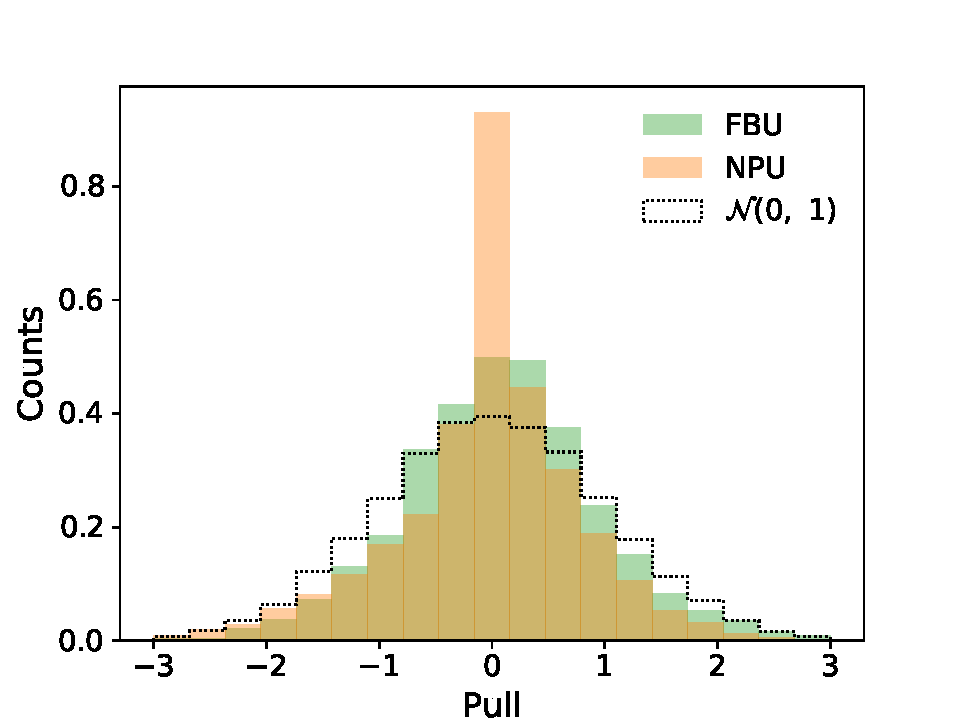
\includegraphics[width=0.48\textwidth]{figures/chapter-04/pulls_smear_0.5_N_100000.pdf}\label{fig:pulls:a}} 
\subfloat[Calibration across smearing parameters]{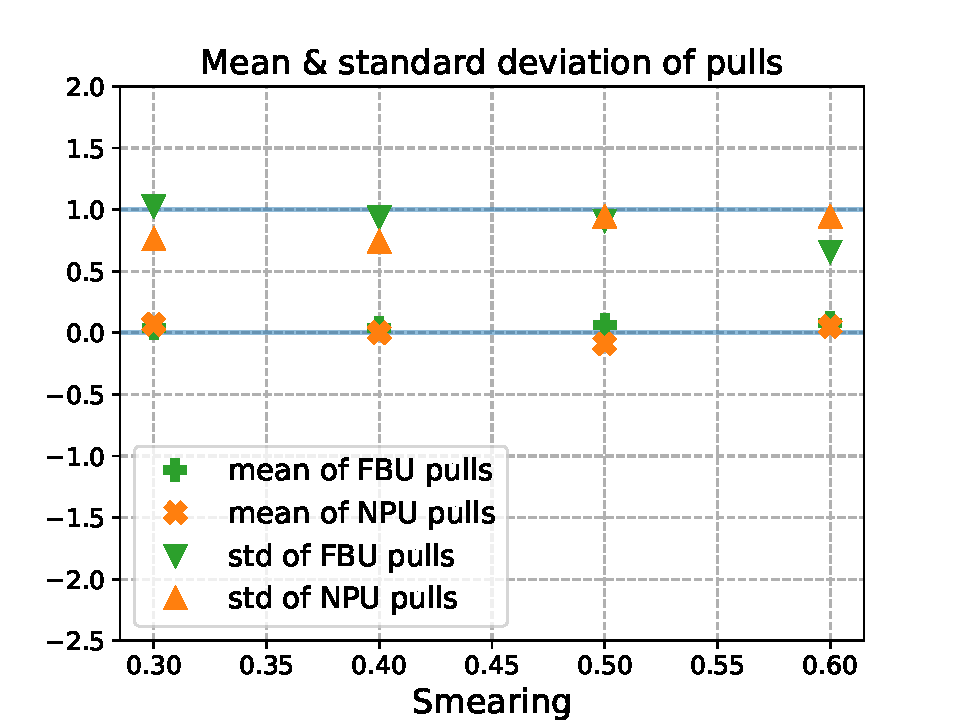
\includegraphics[width=0.48\textwidth]{figures/chapter-04/pulls_mean_std.pdf}\label{fig:pulls:b}} \\
\caption[Statistical calibration analysis for NPU and FBU]{Statistical calibration analysis from 100 pseudo-experiments.
\textbf{(a)} Pull distributions for NPU (orange) and FBU (green) with moderate smearing ($\epsilon = 0.5$), compared against the ideal $\mathcal{N}(0,1)$ reference (black line). 
Both methods show proper calibration with pulls centred at zero and unit variance.
\textbf{(b)} Pull distribution statistics as functions of smearing parameter $\epsilon \in [0.3, 0.6]$. 
The mean and standard deviation remain consistent with the ideal values ($\mu = 0$, $\sigma = 1$) across the range, confirming robust uncertainty quantification for both methods.\footnotemark
}
\label{fig:pulls}
\end{figure}
\footnotetext{Figure created by Jingjing Pan.}

This highlights an important practical advantage of NPU is its computational efficiency for repeated unfolding tasks.
%
In the benchmark with 100 pseudo experiments, FBU using \(\num{10,000}\) MCMC draws requires approximately \(\siqty{40}{\s}\) per experiment, totalling about \(\siqty{67}{\minute}\).
%
NPU requires about \(\siqty{280}{\s}\) for initial training but processes new datasets in just seconds each, yielding a total time of about \(\siqty{5}{\minute}\) for all \(\num{100}\) experiments.
%
This \(\numproduct{13x\,}\) speed-up stems from NPU's amortised inference approach, which eliminates repeated MCMC sampling for new datasets.
%
\cref{tab:timing} summarises the computational cost of NPU and FBU for 100 runs.

\subsection{Particle physics example.}
\begin{figure}
\centering
\subfloat[Jet width $\omega$]{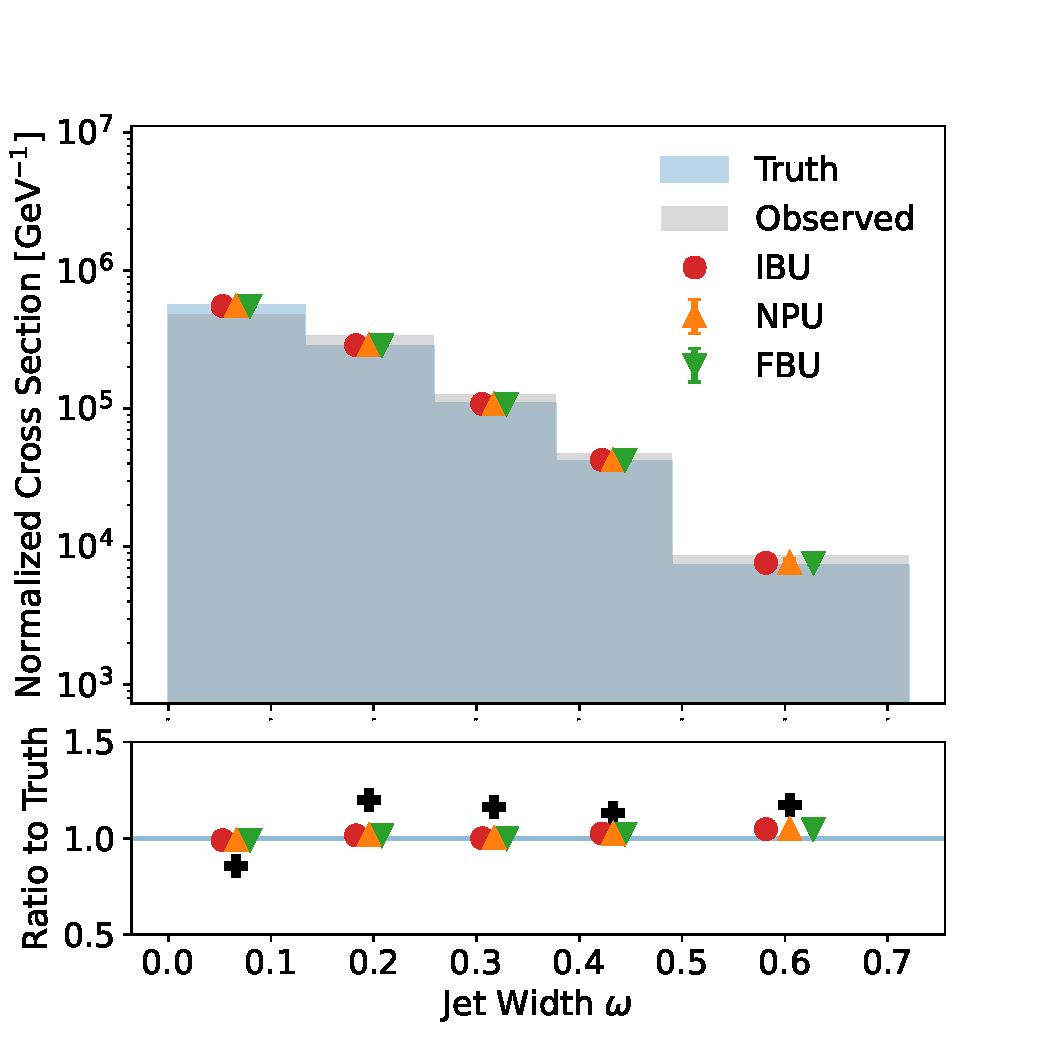
\includegraphics[width=0.46\textwidth]{figures/chapter-04/npu_width_logy.pdf}\label{fig:phys_width}} 
\subfloat[Groomed momentum fraction $z_g$]{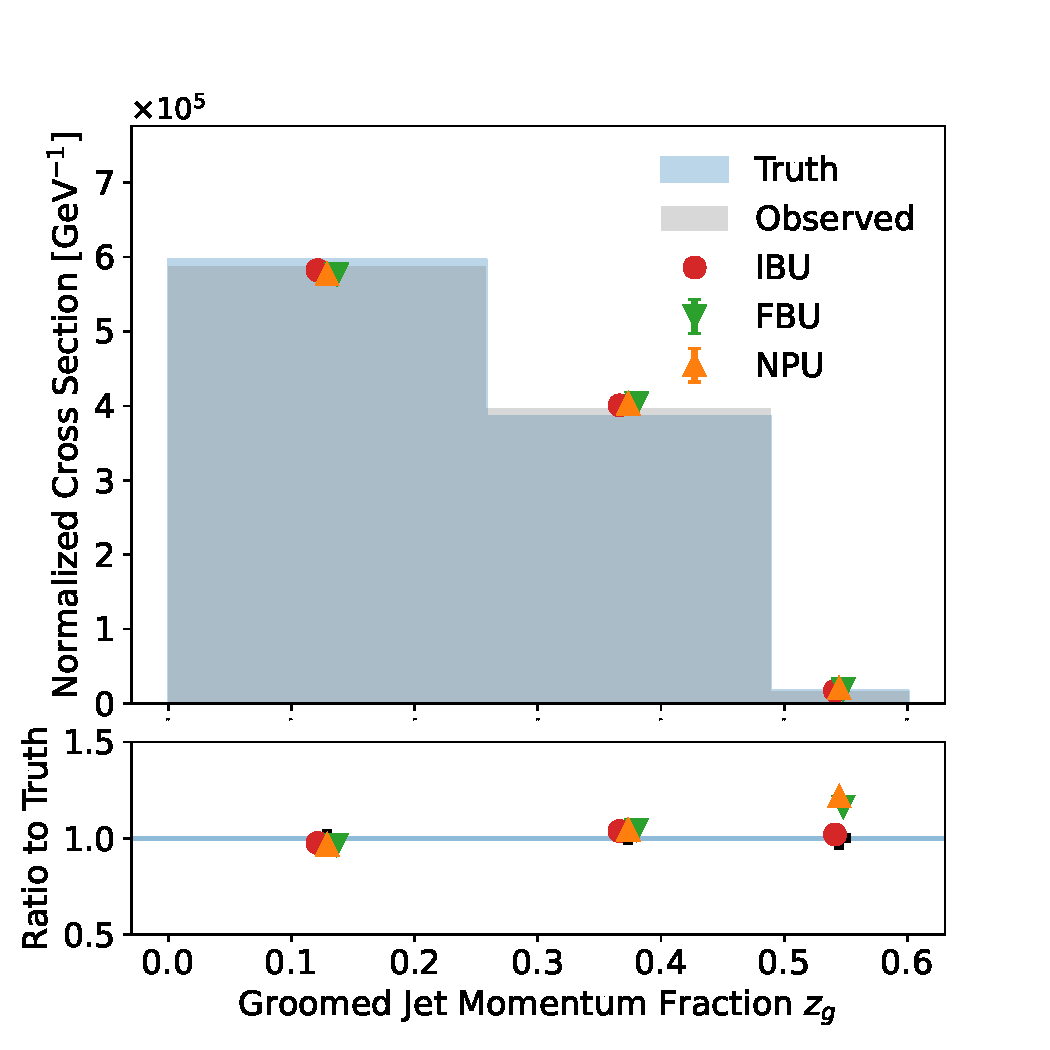
\includegraphics[width=0.46\textwidth]{figures/chapter-04/npu_zgs.pdf}\label{fig:phys_zg}} \\
\subfloat[$N$-subjettiness ratio $\tau_{21}^{\beta=1}$]{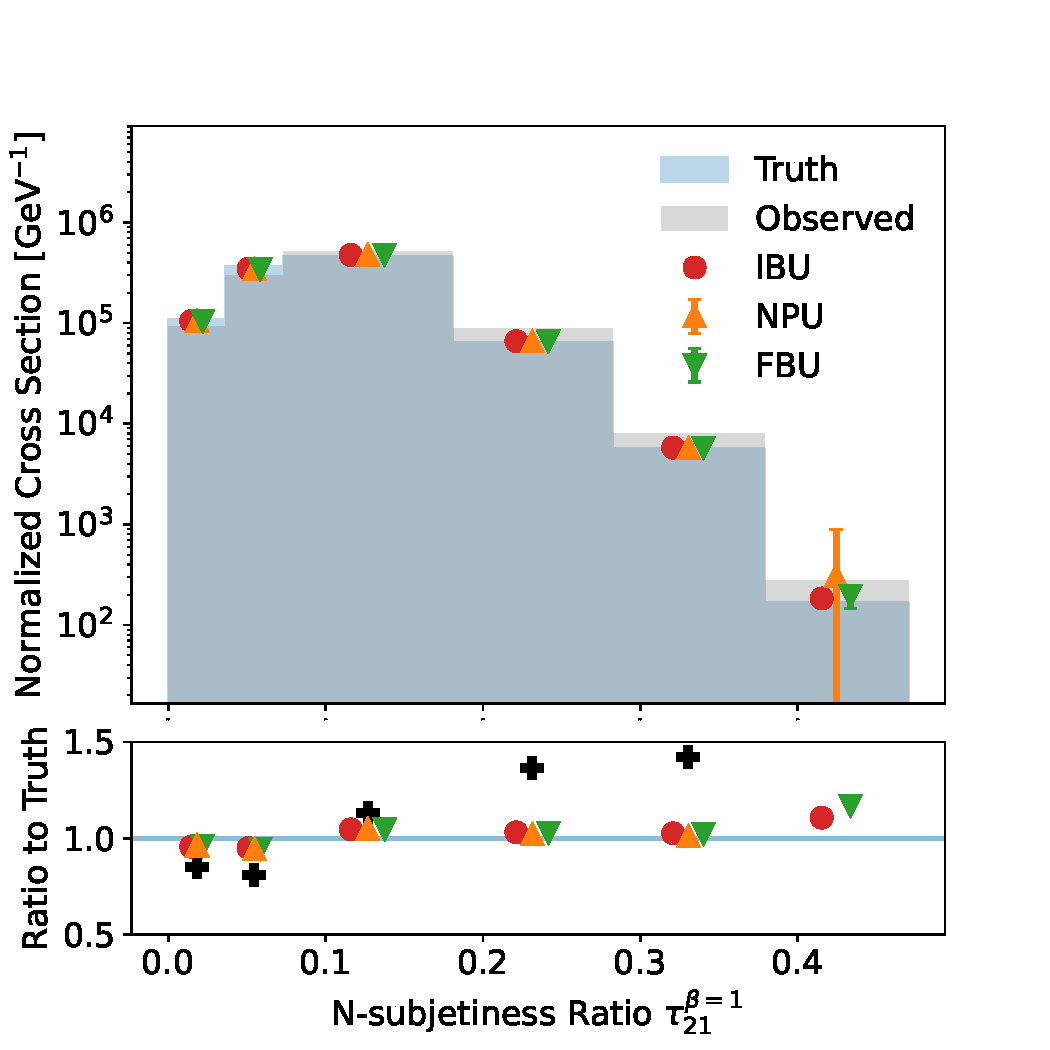
\includegraphics[width=0.46\textwidth]{figures/chapter-04/npu_tau2s_logy.pdf}\label{fig:phys_tau21}} 
\subfloat[Constituent multiplicity $M$]{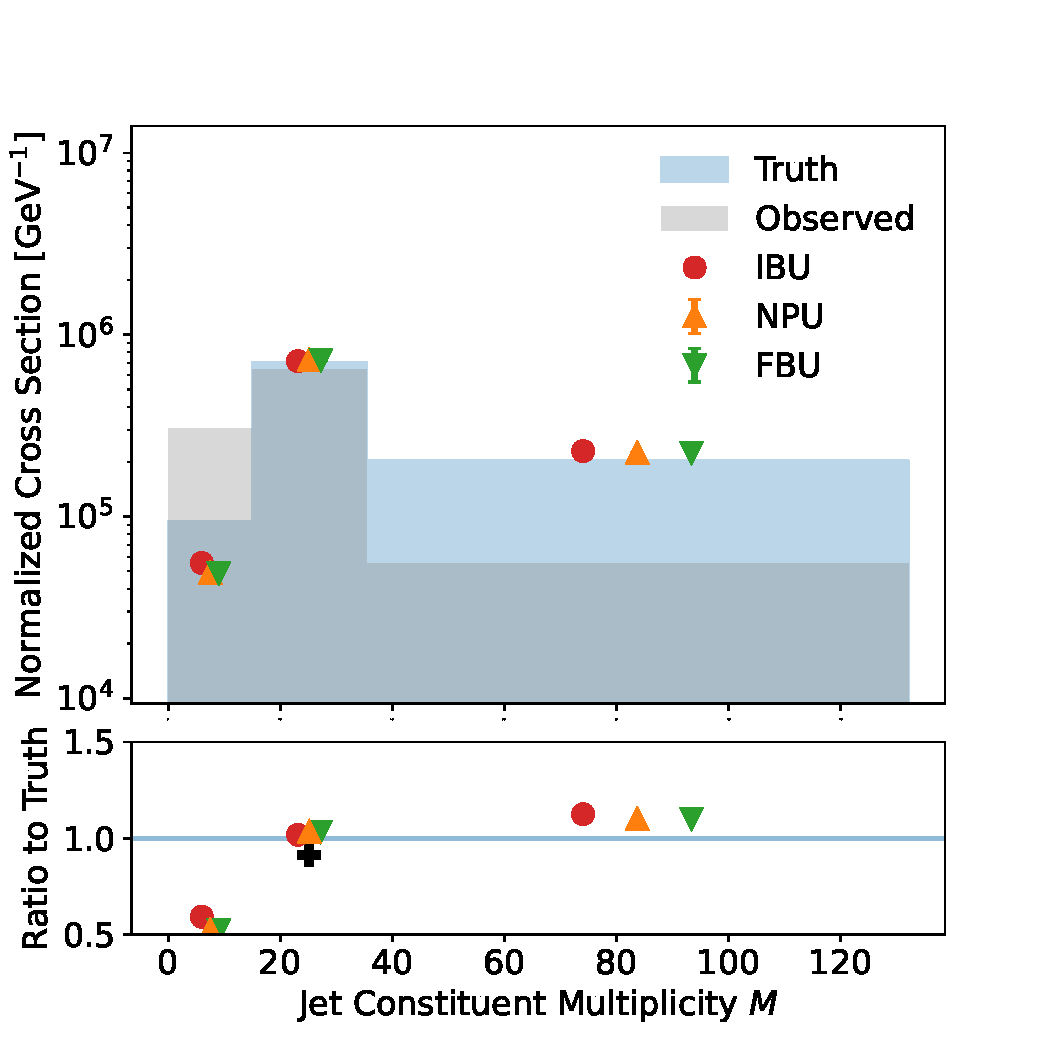
\includegraphics[width=0.46\textwidth]{figures/chapter-04/npu_mult_logy.pdf}\label{fig:phys_mult}} 
\caption[Jet substructure unfolding results using NPU, FBU, and IBU]{Unfolding results for jet substructure observables comparing NPU, FBU, and IBU methods.
The response matrix is constructed using \textsc{Pythia} 8.243 (Tune 21) simulation, while \textsc{Herwig} 7.1.5 provides both the observed data and particle level truth for validation.
%
Truth distributions are shown as blue shaded regions, with unfolded results from NPU (MLE as orange points), FBU (green points), and IBU (red points).
%
Error bars represent posterior standard deviations from the respective methods.
%
NPU successfully recovers the particle level truth distributions across all observables.\footnotemark
}
\label{fig:substructure}
\end{figure}
\footnotetext{Figure created by Jingjing Pan.}

    The final evaluation demonstrates NPU's application to a realistic hig -energy physics scenario, focusing on jet substructure measurements at the Large Hadron Collider (LHC).
    \subsubsection{Dataset and Observables}
        The dataset comprises simulated proton--proton collisions at $\sqrt{s} = 14$ TeV, following the setup in~\cite{andreassen_omnifold_2020}.
        %
        Two simulation generators are employed,
        \begin{itemize}
            \item \textsc{Herwig 7.1.5}~\cite{Bellm2017HerwigNote} serves as the data and truth distributions
            \item \textsc{Pythia 8.243} with Tune 21~\cite{bierlich_comprehensive_2022} is used to construct the response matrices.
        \end{itemize}
        
        Detector effects are emulated using \textsc{Delphes 3.4.2}~\cite{DeFavereau2014DELPHESExperiment}, a fast simulation of the CMS detector with particle flow reconstruction.
        %
        Jets are clustered using the anti$-k_T$ algorithm~\cite{Cacciari2008TheAlgorithm} with radius parameter $R = 0.4$, as implemented in \textsc{FastJet 3.3.2}~\cite{Cacciari2012FastJetManual}.
        %
        To minimize acceptance effects, this analysis includes only the leading jets in events containing a \(Z\) boson with transverse momentum \(p_T^Z > \siqty{200}{\GeV}\).
        %
        After selection, approximately \(\num{1.6d6}\) events from each simulation are retained.

        We focus on four key jet substructure observables that are widely used in LHC analyses.
        \begin{enumerate}
            \item Jet width (\(w\)): the transverse momentum weighted first radial moment of radiation within a jet,
            \item Jet constituent multiplicity ($M$): the number of constituents in a jet,
            \item \(N-\)subjettiness ratio ($\tau_{21} = \tau_2^{\beta=1}/\tau_1^{\beta=1}$): a measure of the compatibility of a jet with a two--prong substructure hypothesis relative to a one--prong hypothesis~\cite{Thaler2011IdentifyingN-subjettiness, Thaler2012MaximizingN-subjettiness, DevNairDevelopmentData}
            \item Groomed momentum fraction ($z_g$): the momentum sharing between sub--jets after soft drop grooming~\cite{Larkoski2014SoftDrop, Dasgupta2013TowardsSubstructure}
        \end{enumerate}
        These observables span a diverse range of physical characteristics and detector sensitivities, providing a comprehensive test of NPU's capabilities.
    \subsubsection{Results}
        \cref{fig:substructure} presents the unfolded distributions for each observable, comparing results from NPU, FBU, and IBU against the known truth.
        %
        For the FBU implementation in this more complex scenario, one needs to increase the number of MCMC steps ten fold compared to the Gaussian example, using \(\num{100000}\) tuning steps and \(\num{500000}\) draws.
        
        For all the observables, NPU accurately recovers the truth, with uncertainty bands that properly account for statistical uncertainties.
        %
        The results demonstrate a few different characteristics of NPU.
        %
        First, NPU effectively handles the complex detector effects present in realistic LHC simulations.
        %
        Second, the method exhibits robustness against simulation modeling differences: the response matrix is constructed using \textsc{Pythia} events, while the ``nature'' distribution NPU was expected to unfold was derived from \textsc{Herwig}, representing different underlying physics models and parton shower algorithms.
        %
        Finally, full posterior information enables rigorous uncertainty quantification across the entire distribution.
        %
        The corner plots for these distributions \cref{fig:phys-corner} reveal the complex correlation structure between bins, information that is typically unavailable with traditional unfolding methods unless explicitly computed via bootstrapping or similar approaches.

        These results highlight NPU's value for practical cross section measurements at HEP experiments, where detector effects are complex and true distributions may differ significantly from simulation.
        %
        In a complete experimental analysis, uncertainties in the response matrix itself could be incorporated either by repeating the unfolding procedure with systematically varied response matrices or by including these systematic uncertainties directly in the likelihood formulation.

\begin{figure}
\centering
\subfloat[Jet width $\omega$]{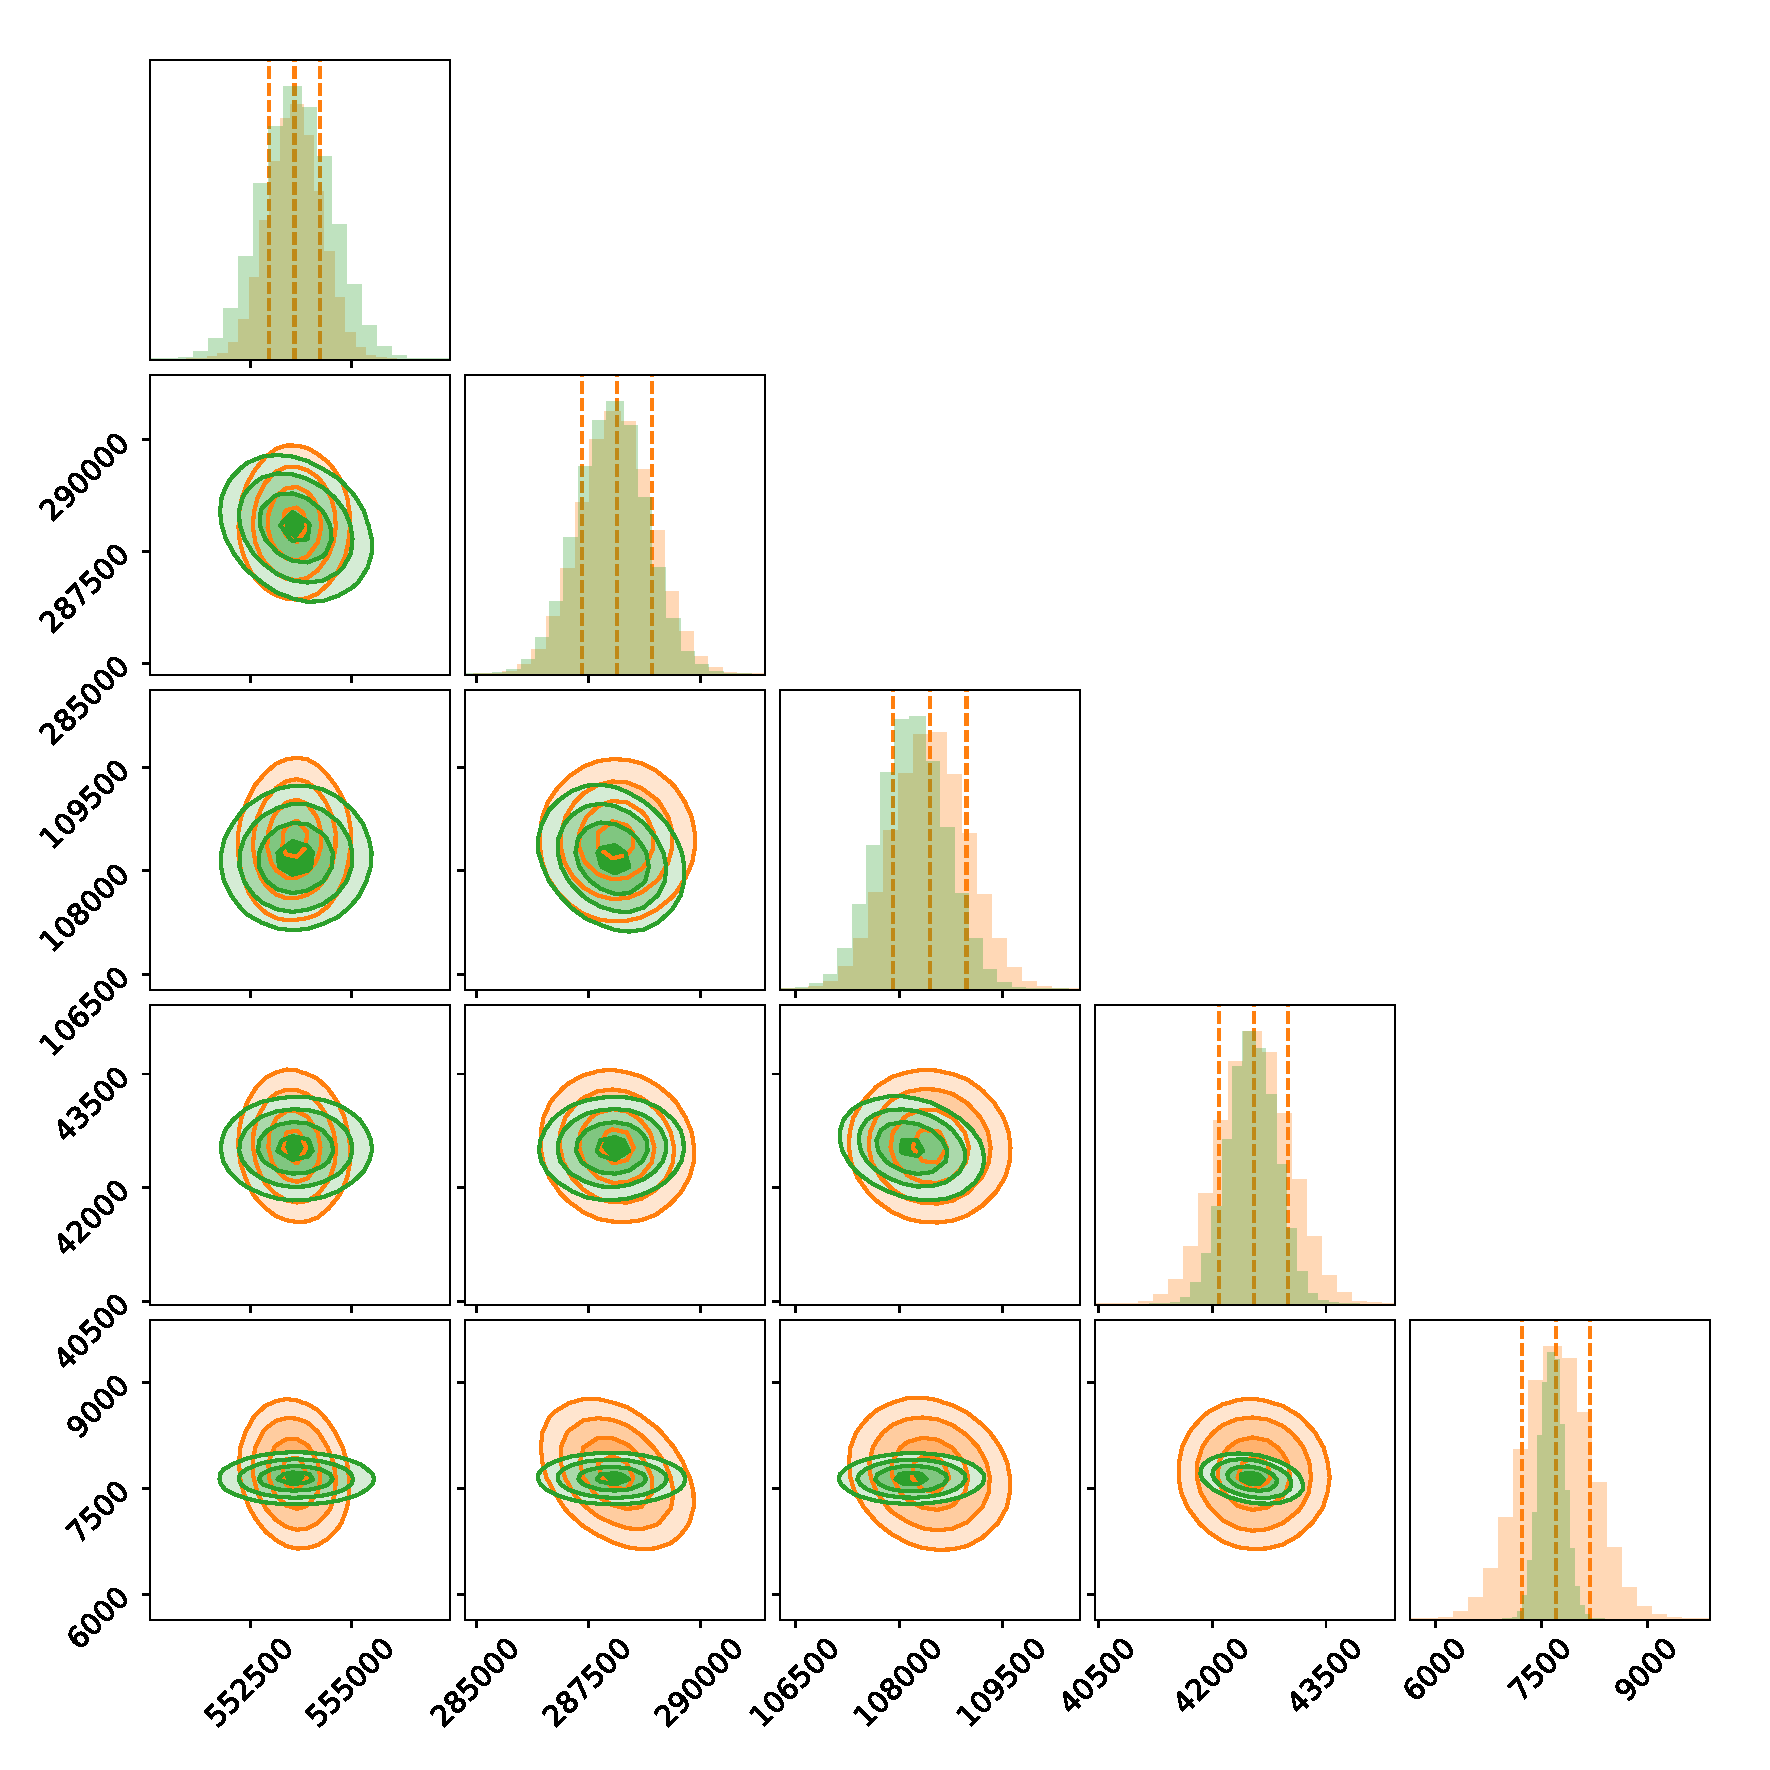
\includegraphics[width=0.45\textwidth]{figures/chapter-04/corner_both_width.pdf}\label{fig:corner_width}} 
\subfloat[Groomed momentum fraction $z_g$]{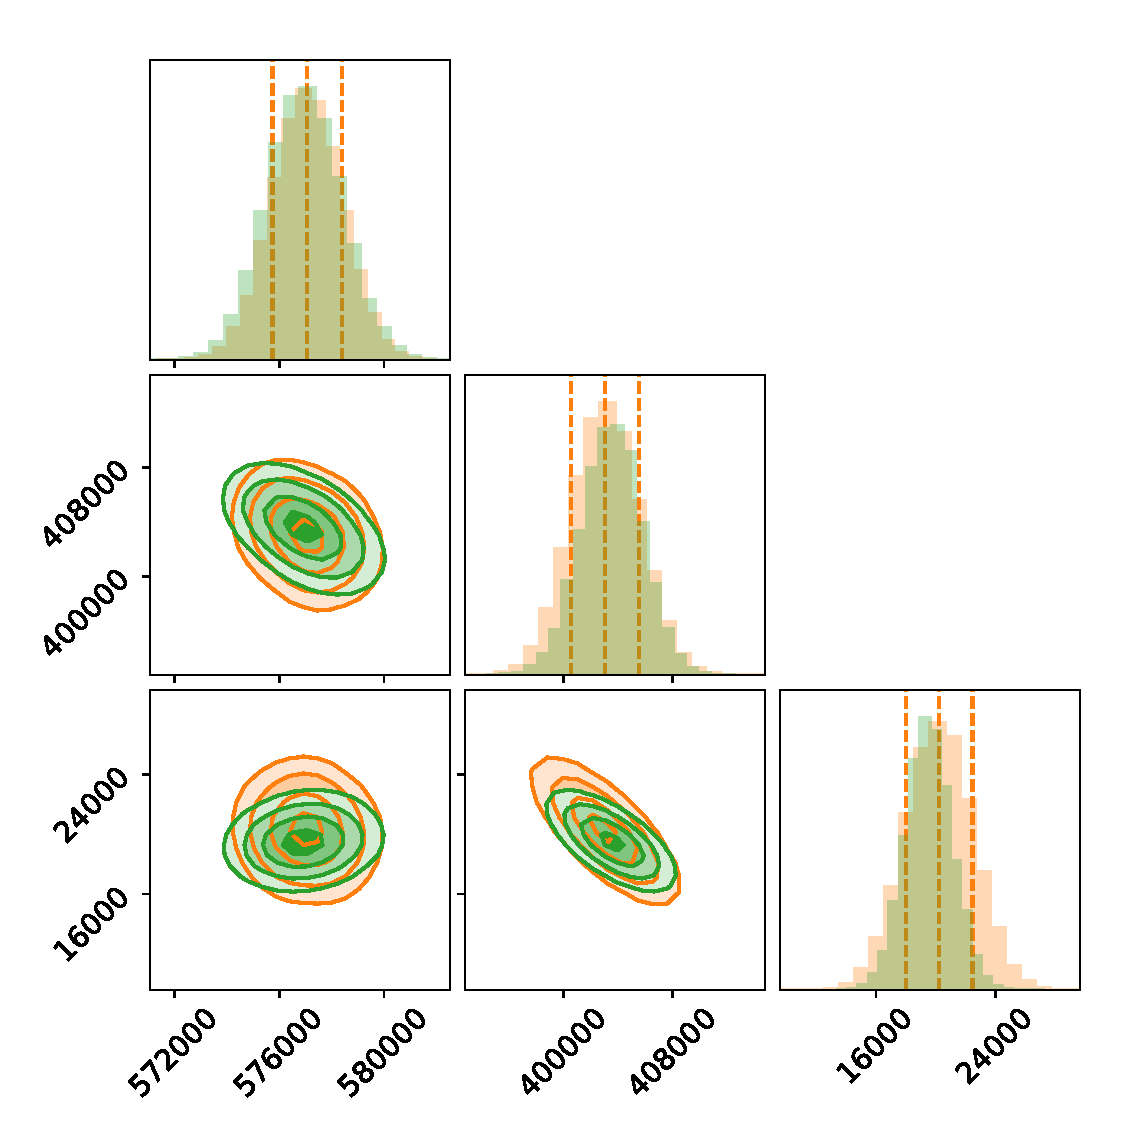
\includegraphics[width=0.45\textwidth]{figures/chapter-04/corner_both_zgs.pdf}\label{fig:corner_zg}}\\
\subfloat[Constituent multiplicity $M$]{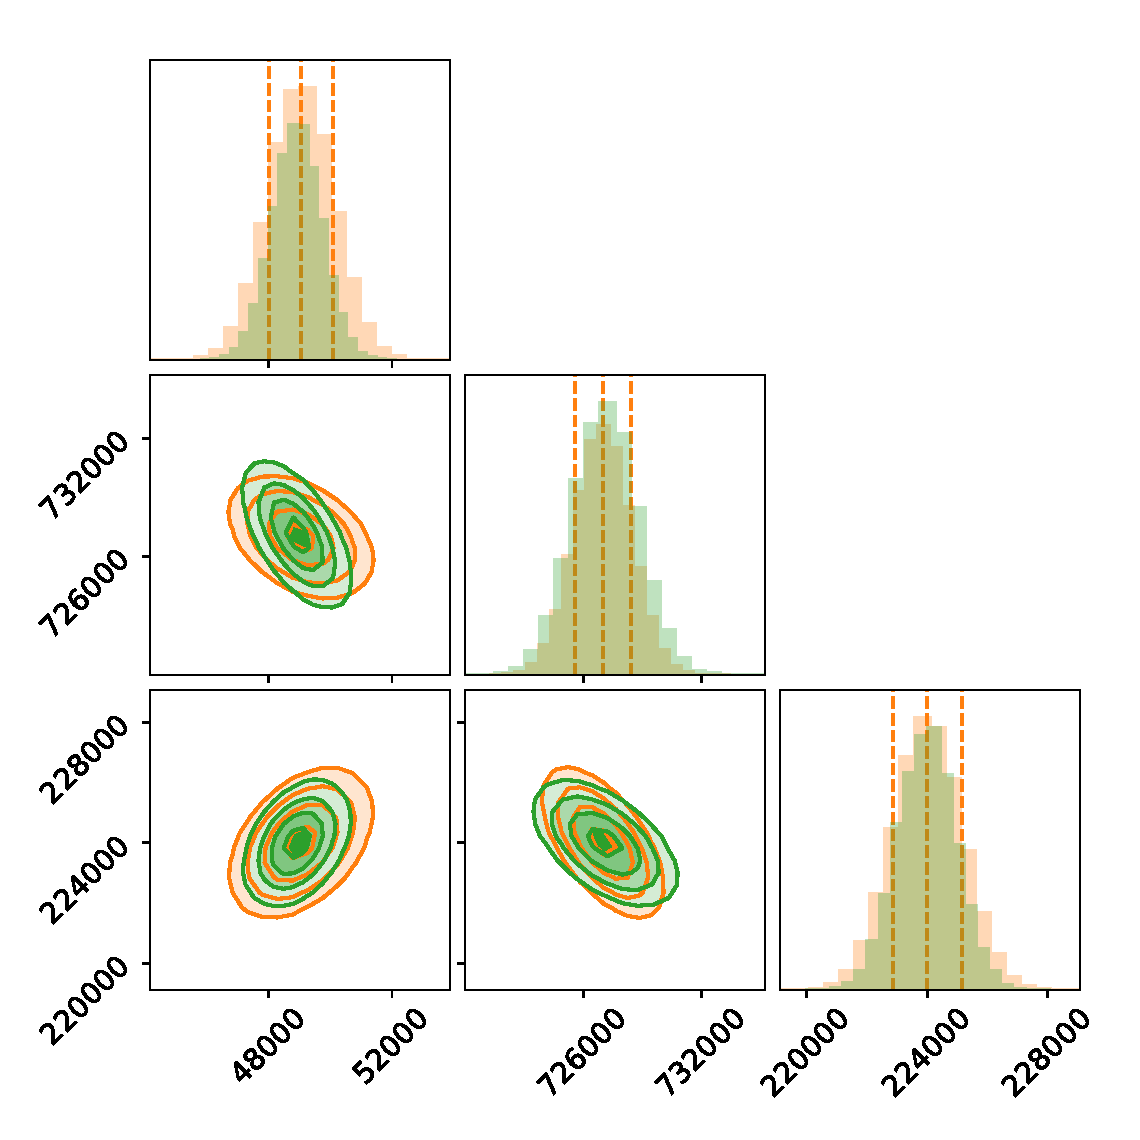
\includegraphics[width=0.45\textwidth]{figures/chapter-04/corner_both_mult.pdf}\label{fig:corner_mult}}
\subfloat[$N$-subjettiness ratio $\tau_{21}^{\beta=1}$]{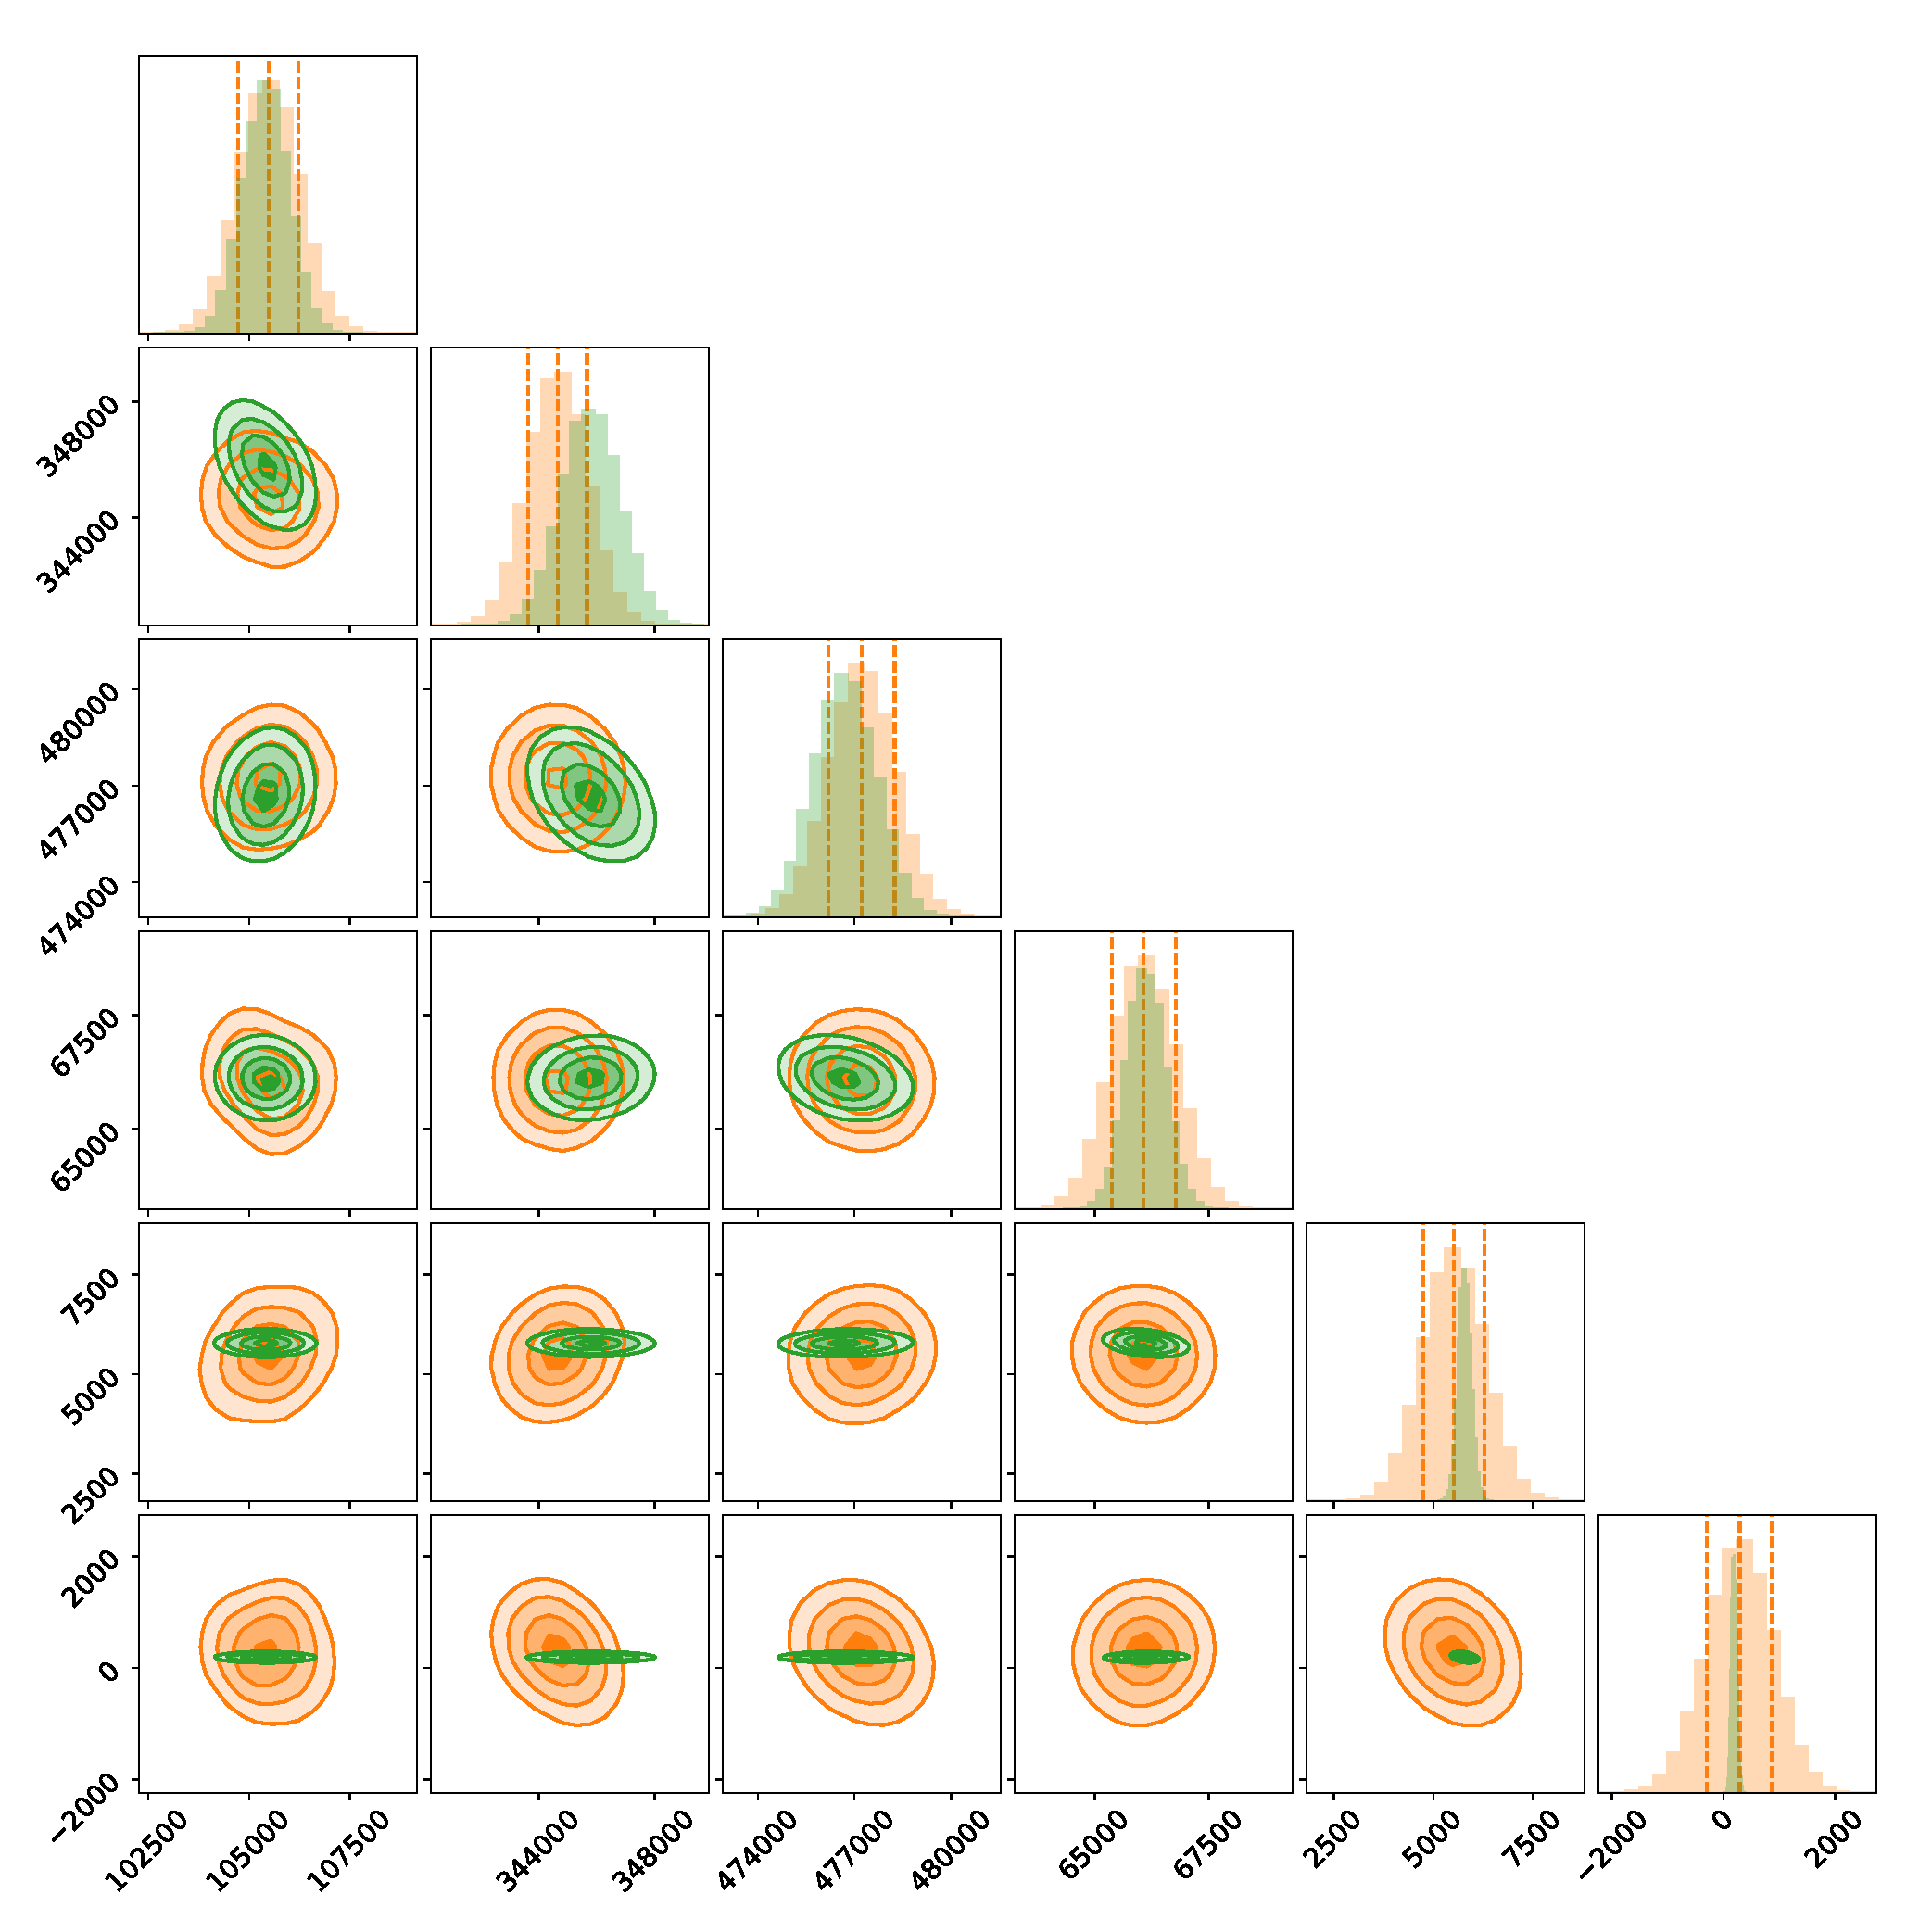
\includegraphics[width=0.45\textwidth]{figures/chapter-04/corner_both_tau2s.pdf}\label{fig:corner_tau21}}
\caption[Corner plots for jet substructure observables]{Corner plots showing posterior correlations for jet substructure observables.
Each panel displays pairwise correlations between bins for one observable, comparing NPU (orange contours) and FBU (green contours, averaged over MCMC samples) posteriors, with truth values marked in blue.
The plots reveal complex bin to bin correlation structures that are typically unavailable from traditional unfolding methods.
Strong agreement between NPU and FBU posteriors confirms the reliability of both approaches, while the encompassing of truth values validates proper uncertainty quantification.
These correlations provide crucial information for propagating uncertainties in downstream physics analyses.\footnotemark
}
\label{fig:phys-corner}
\end{figure}        
\footnotetext{Figure created by Jingjing Pan.}
\subsection{Summary of Numerical Results}
    These numerical studies demonstrate that NPU provides appropriate uncertainty quantification in degenerate scenarios where traditional methods fail, while maintaining proper statistical coverage across varying degrees of detector smearing.
    %
    NPU efficiently processes multiple datasets through amortized inference, and accurately recovers truth distributions in both targeted degenerate toy examples and realistic high energy physics scenarios.
    %
    The method combines the Bayesian foundations of FBU with several architectural and computational advantages.
    %
    The normalising flow architecture can represent a wide range of posterior distributions, including multimodal, asymmetric, and strongly correlated distributions that may be challenging for traditional MCMC methods.
    %
    By providing differentiable access to the posterior density, NPU enables gradient--based optimization for finding maximum likelihood estimates or other derived quantities.

    While FBU requires MCMC sampling for each new measurement, NPU's amortised inference approach front loads computational cost into the training phase.
    %
    Once trained, inference with NPU requires only forward passes through the neural network, making it particularly valuable for analysing large datasets, performing multiple analyses with different systematic variations, bootstrapping for uncertainty estimation, and studies requiring many unfolding runs
    %
    NPU also scales more favourably to high dimensional problems compared to MCMC based methods, which often suffer from the curse of dimensionality and mixing problems in complex posterior landscapes.
    
    However, several limitations should be kept in mind.
    %
    The flexibility of normalising flows comes with increased model complexity, requiring careful architecture design and hyperparameter tuning.
    %
    While less explicit than in traditional methods, NPU's results still depend on the distribution of the generated data, which implicitly defines a prior over the particle level histograms.
    %
    Also, as with any Bayesian method, it is important to validate that the posterior credible intervals have the correct frequentist coverage properties for critical analyses.
    
    Despite these considerations, NPU represents a significant advancement in unfolding methodology, combining the statistical rigour of Bayesian inference with the flexibility and computational efficiency of modern deep learning approaches making it a promising tool for cross section measurements in high energy physics.

\section{Beyond binning: the path forward}
    The Neural Posterior Unfolding method presented in this chapter represents a significant advancement in binned unfolding approaches.
    %
    By incorporating normalising flows for posterior estimation, NPU addresses several limitations of traditional methods while maintaining the established binning paradigm that has served particle physics for decades.
    %
    However, binning itself introduces fundamental constraints that motivate the development of alternative, unbinned methodologies.

    Binning inherently discards information about the precise location of events within each bin, reducing statistical precision.
    %
    The mantra ``The choice of binning is subjective and can introduce biases in the unfolded results'' is oft expressed in statistical treatments of the unfolding problem~\cite{cowan_survey_2002, cowan_statistics_2021, CowanStatisticalRehovot, Cowan2011AsymptoticPhysics,Tang2017DataMethod, hocker_svd_1996, Gagunashvili2024DataOptimization, CranmerPracticalLHC, StatisticalPhysics, Bohm2025IntroductionPhysicists, gardi_statistics_2015, Adam-Bourdarios2015TheChallenge, cowan_topics_2010}.
    %
    This discretisation is particularly problematic for observables with sharp features or resonances that may be obscured by bin boundaries.
    %
    The restrictions the curse of dimensionality imposes on binned methods' applicability to multivariate problems has already been discussed, 

    Binned methods require separate unfolding procedures for each differential distribution of interest.
    %
    This approach is inefficient when multiple observables derived from the same dataset need to be unfolded, as is common in comprehensive physics analyses.
    
    Recent years have seen the rapid development of unbinned unfolding methods powered by advances in deep learning.
    %
    These innovations have enabled significant progress towards solving the challenges posed by binned methods.
    %
    Although machine learning methods are typically a few orders of magnitude slower than traditional methods like IBU, modern ML techniques can leverage efficient data representations and parallelised computation for faster inference, reducing the gap particularly for high dimensional problems.

    The next chapters will explore some unbinned methods in detail, examining their theoretical foundations, practical implementations and performance characteristics on realistic physics examples.
    %
    These methods build upon the insights from binned approaches like NPU while overcoming the intrinsic limitations of binning to enable new capabilities for precision measurements in high energy physics.
    %
    As experimental datasets grow larger and theoretical predictions become more precise, unbinned methods will play an increasingly important role in extracting the full physics potential from experiments.
    %
    The transition from binned to unbinned unfolding represents not just a technical evolution but a paradigm shift in how we approach the measurement and interpretation of cross section measurements.